\documentclass[11pt,twoside]{eitExjobb}
%\documentclass[11pt,twoside,final]{eitExjobb}  % Use final for the final version that will be printed
%%%%%%%%%%%%%%%%%%%%%%%%%%%%%%%%%%%%%%%%%%%%%%%%%%%%
%% Other fonts (Palatino as rm font, helvetica as sf font and courier as tt font. All fonts are normally installed with a standard LaTeX distribution.)
% \usepackage{mathpazo} % Also in math mode
% \usepackage[scaled=.95]{helvet}
% \usepackage{courier}
%%%%%%%%%%%%%%%%%%%%%%%%%%%%%
%
\usepackage[utf8]{inputenc}  % Input encoding (this file): 8 bit unicode.
\usepackage[T1]{fontenc}     % Output encoding (pdf file)
%%%%%%%%%%%%%%%%%%%%%%%%%%%%%
%% Packages used
\usepackage{graphicx}   % Included graphics and some resizable boxes
\usepackage{url}        % nice urls with line breaks 
\usepackage{lipsum}     % nonsense text blocks
\usepackage{booktabs}   % nicer table rules
\usepackage[version=4]{mhchem}   % fancy chemical notation
\usepackage{siunitx}    % better unit notation
\DeclareSIUnit{\torr}{Torr}
\usepackage{fancyref}   % improved labels
\usepackage{parskip}    % better paragraph splitting
\usepackage{subcaption} % easier labeling of subfigures
\usepackage{floatrow}   % for setting table fontsize
%%%%%%%%%%%%%%%%%%%%%%%%%%%%%%
\patchcmd{\thebibliography}{\section*{\refname}}{}{}{}

\DeclareFloatFont{small}{\small}
\floatsetup[table]{font=small}
\floatsetup[table]{style=plaintop}
%%%%%%%%%%%%%%%%%%%%%%%%%%%%%%
%%%%%%%%%%%%%%%%%%%%%%%%%%%%%%
\begin{document}
%%% Title page
\Title{Flashlamp Annealing for Improved Ferroelectric Junctions}
\Author{Theodor Blom\\\texttt{nat13tbl@student.lu.se}}
\Supervisor{Mattias Borg}
\CoSupervisor{Rainer Timm}
\Examiner{Mathieu Gisselbrecht}
\Info{12 months, 60 hp}
%% Set by default
% \Date{\today}    %% Today's date
% \Year{\the\year} %% This year shown in copyright
% \Company{Department of Electrical and Information Technology\\Lund University}
%%%%%%
\MakeTitlePage{}  %%% Print title page and copyright page
%%%%%% 
\frontmatter    %%% Page numbering for front pages (small roman)
%%%%% Abstract
\chapter*{Abstract}

%%%%% Popular Science Summary
\chapter*{Popular Science Summary}
\subsection*{A New Frontier of Computing}
We all recognize the feeling of panic when your computer crashes and you realize
you forgot to save your progress for the past couple of hours. In this scenario
you wait for the computer to boot again and assess what you have lost. Imagine
instead the computer booting instantly and you find yourself exactly where you
left off. With an emerging technology in computer design this could become the
new reality.

The basic idea behind the fundamental building block of your electronic devices,
known as the transistor, has since its invention in the 1960s been largely
unchanged. The design which proved most successful is known as the
Metal-Oxide-Semiconductor Field Effect Transistor (MOSFET) and is by far the
most common design even to this day due to its cheap manufacturing process and
its ability to be scaled down to ever smaller devices. However, in the last
decade one has started to reach the limits of the MOSFET design, primarily due
to limited scalability, and alternative designs are actively being explored.

A promising design is the Ferroelectric Tunnel Junction (FTJ) which utilizes the
small dimensions of the transistor to its advantage where electrons tunnel
through a thin barrier. This barrier is then manipulated to either allow
electrons though or not, resulting in the characteristic transistor
functionality. In addition to being intrinsically small, the ferroelectric
barrier allows the transistor to be toggleable where the state of the transistor
is maintained even though power is lost. This ability means that electronic
devices utilizing this design does not have to be booted up, as all transistors
are already set to the desired state. Additionally, as power is only consumed as
transistors are being toggled between states, these devices could reduce power
consumption lengthening the battery life across all devices.

However, for this to become the new reality of computers, the FTJ design must be
improved further to prove as an effective alternative to the MOSFET design. One
limiting factor is believed to be the interfaces of the ferroelectric barrier
layer. Utilizing a new technique known as Flash-Lamp Annealing (FLA) the
processing of the ferroelectric barrier layer can be made up to 10 000 times
faster which could significantly improve the interfaces. This as the material
can set much faster resulting in better defined interfaces. If successful, this
could be a crucial step for this new transistor design to become a viable
alternative to MOSFETs and bring in a new frontier of computing.

%% ToC etc
\tableofcontents
\listoffigures
\listoftables
\cleardoublepage{}
%%%%% Page numbering for the main thesis (arabic)
\mainmatter{}
%%%%%%%%%%%%%%%%%%%%%%%%%%%%
\chapter{Introduction}\label{ch:intro}

Mål: Introducera området och ge en överblick.\cite{athle2019development}
    
%%%%%%%%%%%%%%%%%%%%%%%%%%%
\chapter{Semiconductors and Ferroelectrics}\label{ch:semiandferro}

Mål: Klargöra varför III-V (utgå från Si) och FE är intressant. Varför gör vi detta? Vad är applikationern? Få med FTJ här!

\section{Ferroelectricity}

Mål: Basics of FE;\  Polarisation, Domäner och PE-kurvor.

\subsection{\ce{HfZrO2}}

Mål: Redogör för FE-\ce{HfO2} och beskriv hur \ce{Zr} kommer in i bilden. Få med
de olika kristallstrukturerna (faser) här.

\subsection{Capping Using \ce{TiN}}

Mål: Få med att capping suppressar den monocliniska fasen och att det är najs.

\section{III-V Semiconductors}

Mål: Redogör för varför III-V är intressant. Direkt bandgap, lägre DOS --> FTJ

\section{The FTJ Structure and Operation}

Mål: Med FE och III-V förklarat, sammanställ allt i hur en FTJ ser ut och
fungerar med banddiagram och allt.

\subsection{Tunneling and Leakage Mechanics}

Mål: Nämn de olika leakage mechanics i FTJ strukturen. Vi vill helst bara ha
direct tunneling.

\subsection{Thermal Budget and Defects}

Mål: Redogör för vilka typer av defekter vi vill åt och hur de påverkas av
thermal budget. As/In diffusion --> Time dependent --> FLA

%%%%%%%%%%%%%%%%%%%%%%%%%%%
\chapter{Fabrication}\label{ch:fab}

Metal-Ferroelectric-Semiconductor capacitors with are to be fabricated using
traditional techniques. The MFS-caps were fabricated in a stack of
\ce{InAs}/\ce{HZO}/\ce{TiN} with an \ce{Au} contact on top. All fabrication was
done at Lund NanoLab (LNL) and is outlined in section \ref{sec:FabProc}. After
fabrication the resulting capacitors have the parameters as stated in table
\ref{tab:fab_param} and look like the picture in figure \ref{fig:fab_babycomp}.

\begin{table}[htbp]
    \centering
    \caption{Relevant fabrication parameters of the samples. Growth and
    annealing parameters of each sample is stated in Chapter
    \ref{ch:res}.}\label{tab:fab_param}
    \begin{tabular}{crc}
        \toprule
        Layer & Thickness & Doping \\\midrule
        \ce{Au} & \SI{200}{\nano\meter} & - \\ 
        \ce{TiN} & \SI{10}{\nano\meter} & - \\ 
        \ce{HfZrO2} & \SI{10}{\nano\meter} & 1:1 (\ce{Hf/Zr}) \\ 
        \ce{InAs} & \SI{280}{\micro\meter} &
        \SI{1e16}{\per\centi\meter\tothe{3}} \\\bottomrule 
    \end{tabular}
\end{table}

\begin{figure}[htbp]
    \centering
    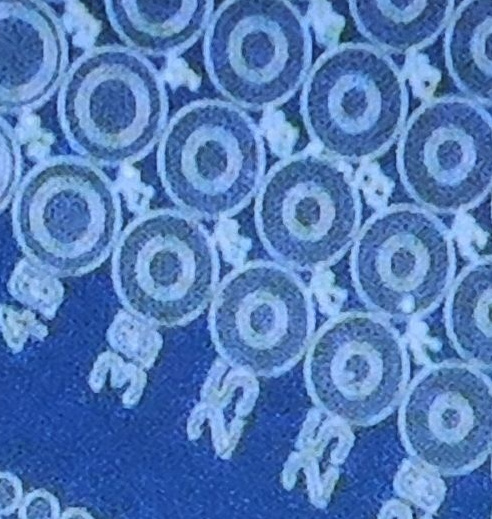
\includegraphics[width=.30\linewidth]{fig/babycomputers.jpg}
    \caption{Picture of fabricated capacitor rings. The numbering refers to the
    diameter of the inner capacitor circle in
    \si{\micro\meter}.}\label{fig:fab_babycomp}
\end{figure}

% \section{Processing Methods}\label{sec:methods}
%
% \subsection{Atomic Layer Deposition (ALD)}
% Atomic layer deposition (ALD) was used to grow the \ce{Hf_xZr_{1-x}O2} layer
% (HZO).
%
% \begin{figure}[htbp]
%     \centering
%     \includegraphics[width=.45\linewidth]{example-image}
%     \caption{Schematic image of the ALD experimental setup. Maybe steal from
%     another paper?}\label{fig:fab_ALDsetup}
% \end{figure}
%
% \subsection{Flash Lamp Annealing (FLA)}
% Flash lamp annealing (FLA) was used to crystallize the HZO to the ferroelectric
% orthorhombic phase.
%
% \begin{figure}[htbp]
%     \centering
%     \includegraphics[width=.45\linewidth]{example-image}
%     \caption{Schematic image of the FLA experimental setup. Should include the
%     most important parts such as flashlamps, sample location, preheating
%     elements and pyrometer.}\label{fig:fab_FLAsetup}
% \end{figure}

\section{Sample Fabrication Process}\label{sec:FabProc}

% Mål: Redogör för hela min process.
% 1. Split wafers
% 1. BOE etch
% 2. ALD
% 3. Sputter TiN
% 4. Annealing
% 5. Spincoat
% 5. Lithography
% 5. Develop structure
% 5. Evaporate Au
% 5. Lift-off
% 6. TiN etch

\subsection{InAs Wafer Preparation}
The initial substrate was a low doped \ce{InAs} \SI{4}{\inch} wafer with a
layer of \ce{In} and \ce{As} oxides on top. Since the wafer is to be used as
bottom contact of our capacitors a wet etch was required before any film
deposition was possible. The wafer was etched in 10:1 \ce{HCl} acid for
\SI{30}{\second} and rinsed in deionized \ce{H2O} to remove any oxides. The
samples were dried using a nitrogen gun and promptly advanced to the next step
to reduce reoxidation. This process is schematically showed in figure
\ref{fig:fab_1}. Before etching the wafers were cut into squares with a side
length of roughly \SI{10}{\milli\meter} to simplify processing.

\begin{figure}[htbp]
    \centering
    
\includegraphics[width=.70\linewidth]{fig/fabproc/fab_1.png}
    \caption{Schematic figure of the sample oxide etching process.}\label{fig:fab_1}
\end{figure}

\subsection{\ce{HfZrO2} Deposition}
With the native \ce{InAs} oxides removed the deposition of \ce{Hf_xZr_{1-x}O2}
was done using atomic layer deposition (ALD) in a Picosun Sunale R-100 system.
Samples were grown using alternating cycles (1:1) of TEMA(Hf) and TEMA(Zr)
precursors to achieve equal distribution of \ce{Hf} and \ce{Zr} ($x=0.5$) in
the resulting $\sim$\SI{10}{\nano\meter} oxide. Depending on the sample series
both chamber temperature and the number of cycles were altered. The specific
growth parameters for each samples is specified in Appendix \ref{app:procparam}.
Figure \ref{fig:fab_2} shows a schematic of the samples at this fabrication
stage.

\begin{figure}[htbp]
    \centering
    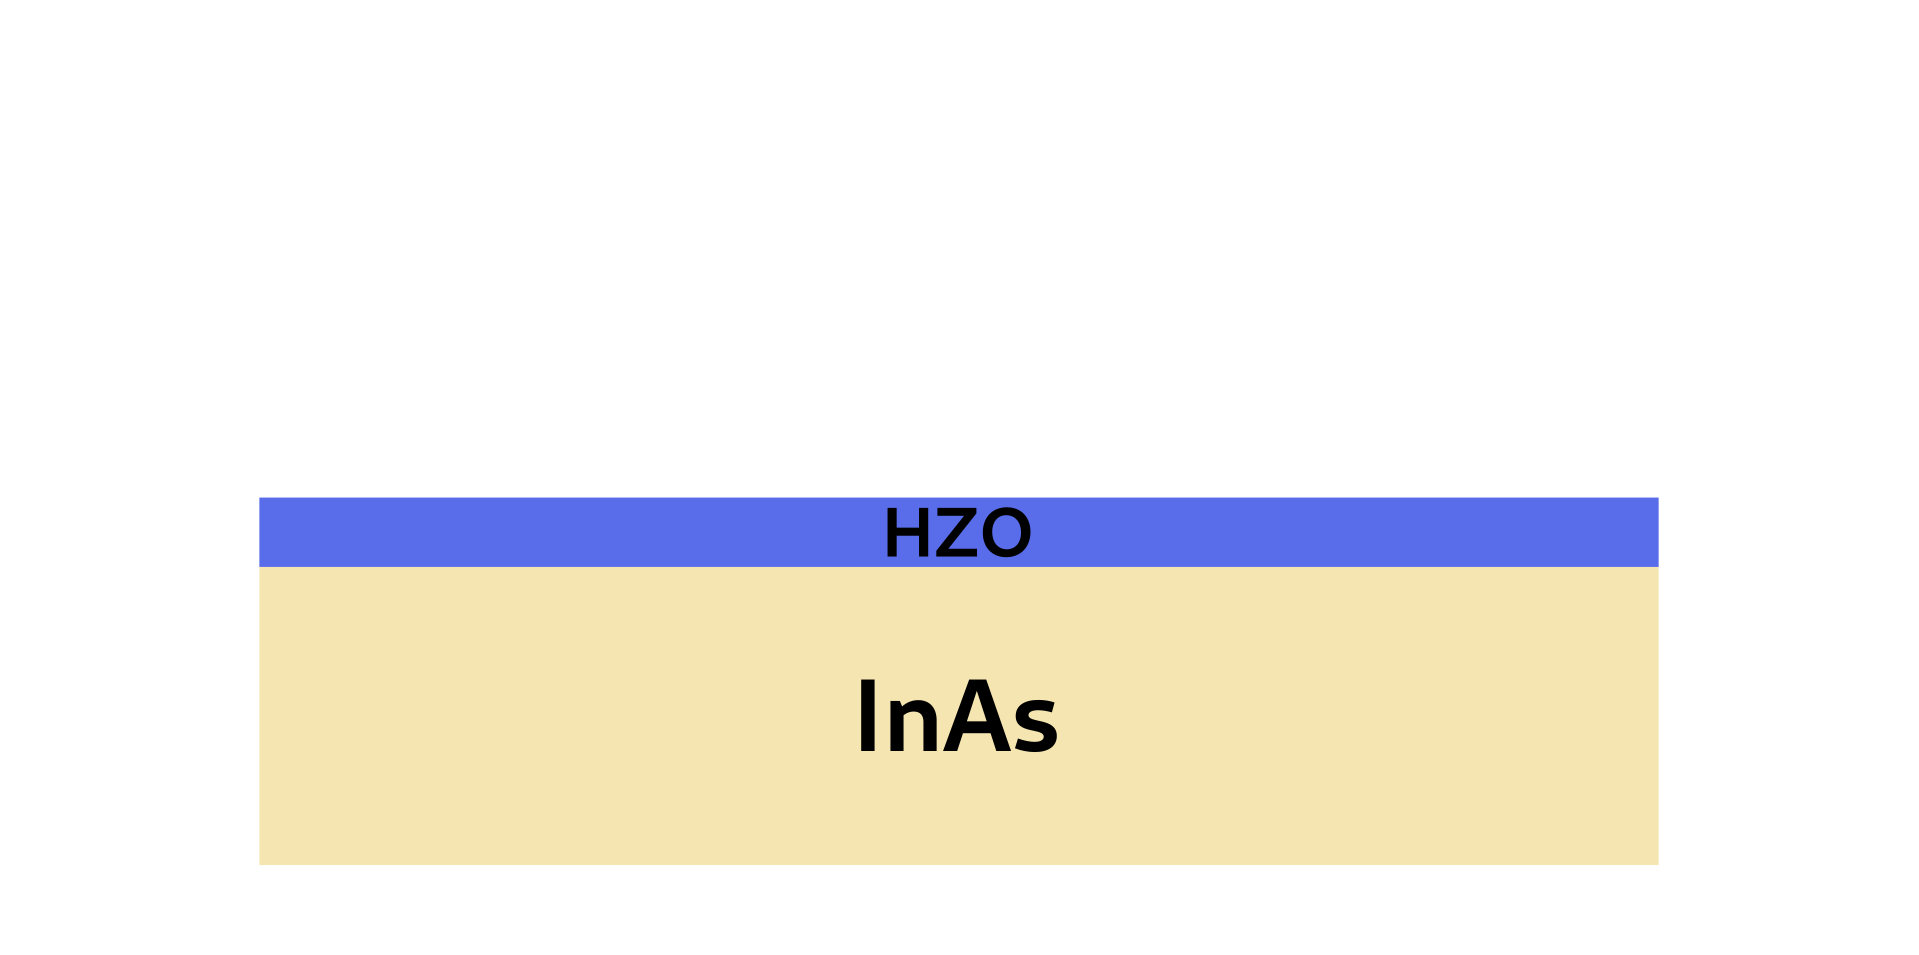
\includegraphics[width=.45\linewidth]{fig/fabproc/fab_2.png}
    \caption{Schematic figure of the sample after atomic layer
    deposition.}\label{fig:fab_2}
\end{figure}

\subsection{Top Electrode Deposition}
After deposition of the \ce{HfZrO2} film, a $\sim$\SI{10}{\nano\meter} top
contact of \ce{TiN} was deposited through sputtering using an AJA Orion 5
sputter machine. Pumping the chamber to <\SI{2.7}{\milli\torr} and pre-cleaning
the source for \SI{5}{\minute} the samples were sputtered at a power of
\SI{150}{\watt}. Sputtering for $\sim$\SI{11}{\minute} at a deposition rate of
\SI{0.15}{\nano\meter\per\second} resulted in the desired layer thickness.
Figure \ref{fig:fab_3} shows a schematic of the samples at this stage of
fabrication.

\begin{figure}[htbp]
    \centering
    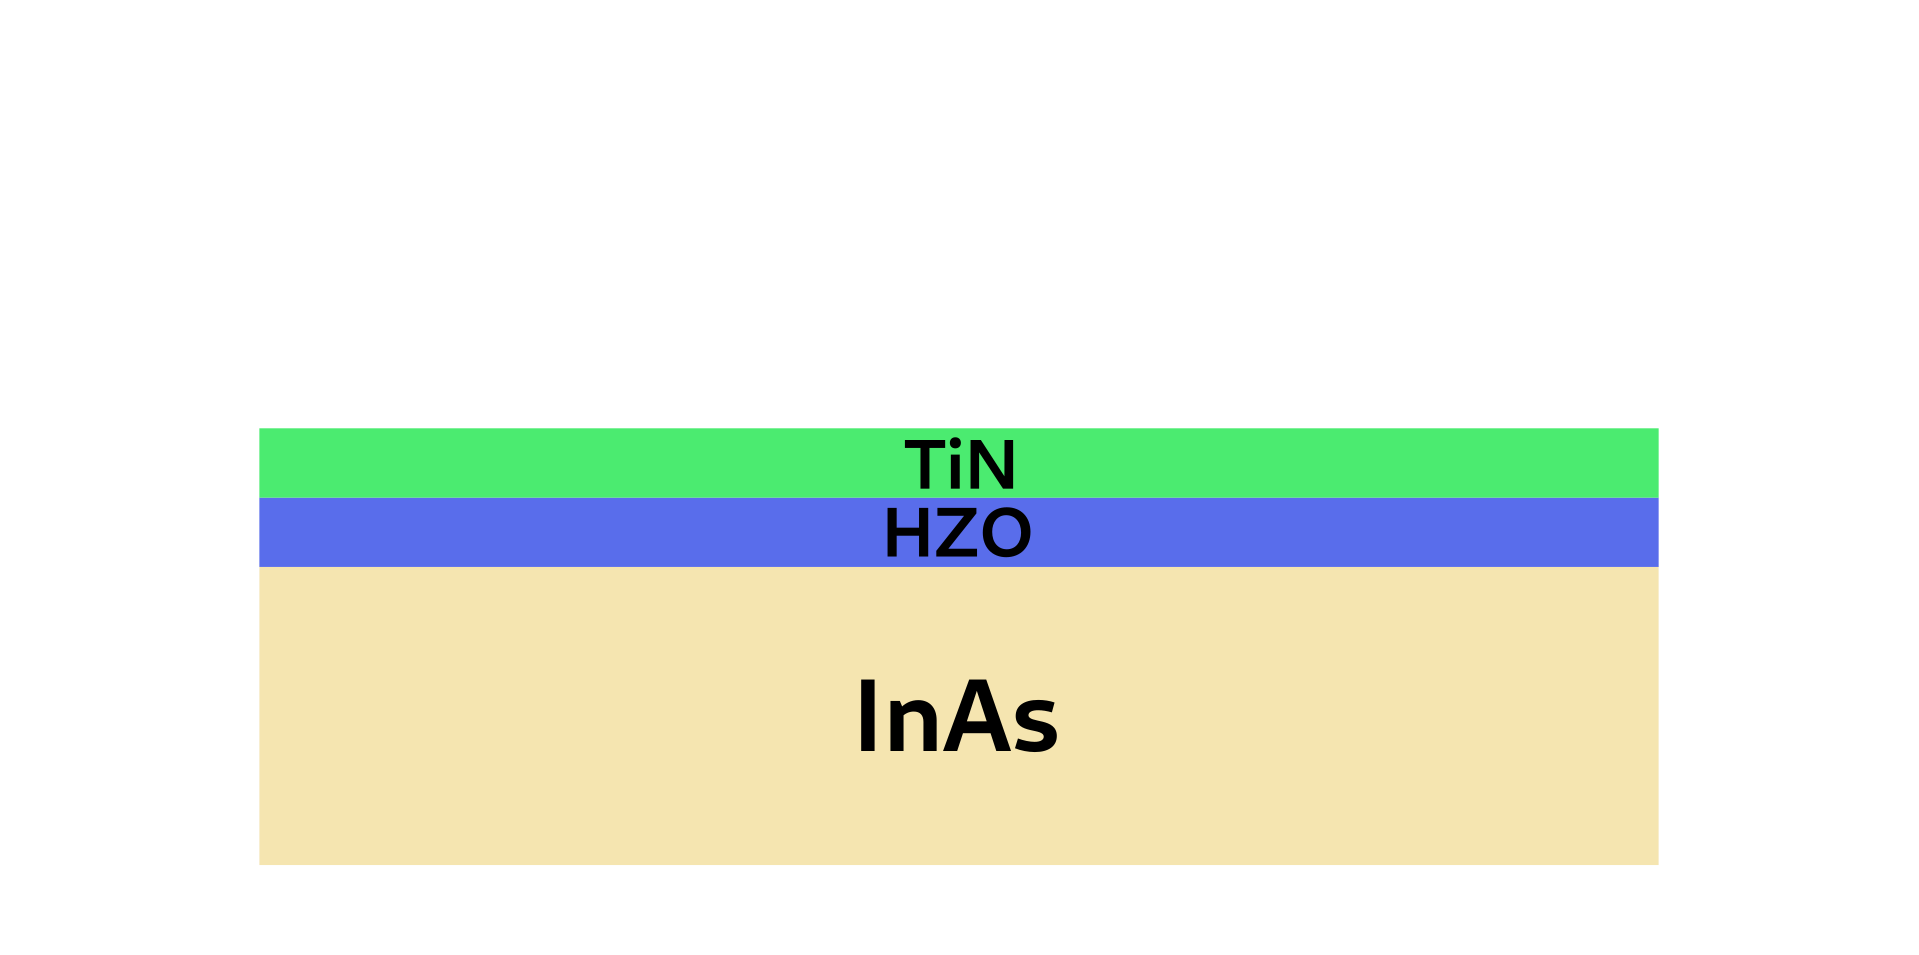
\includegraphics[width=.45\linewidth]{fig/fabproc/fab_3.png}
    \caption{Schematic figure of the sample after top contact
    sputtering.}\label{fig:fab_3}
\end{figure}

\subsection{Annealing Process}
With the amorphous oxide contained between the bottom- and the top contact annealing
could take place. Depending on the sample annealing was either done through
rapid thermal processing (RTP) or flash lamp annealing (FLA). The reference RTP
sample were annealed at \SI{600}{\celsius} for \SI{30}{\second} in a
RTP-1200-100 system from UniTemp GmbH while all other samples were annealed in
the FLA system by \SI{5}{\milli\second} pulses of varying energy and number.
See figure \ref{fig:res_Comsol} and Appendix \ref{app:procparam} for a detailed
overview of the number of flashes per sample and their energies.

\subsection{Metal Contacting}
In order to electrically characterize the samples, individual devices would
have to be defined as well as covered in thicker highly conductive \ce{Au} to
not damage the underlying structure using the probe techniques described in
Chapter \ref{ch:char}. The devices were defined using optical lithography and
the \ce{Au} was deposited using electron-beam evaporation. Figure
\ref{fig:fab_4} shows a schematic of the samples at this stage of fabrication.

\begin{figure}[htbp]
    \centering
    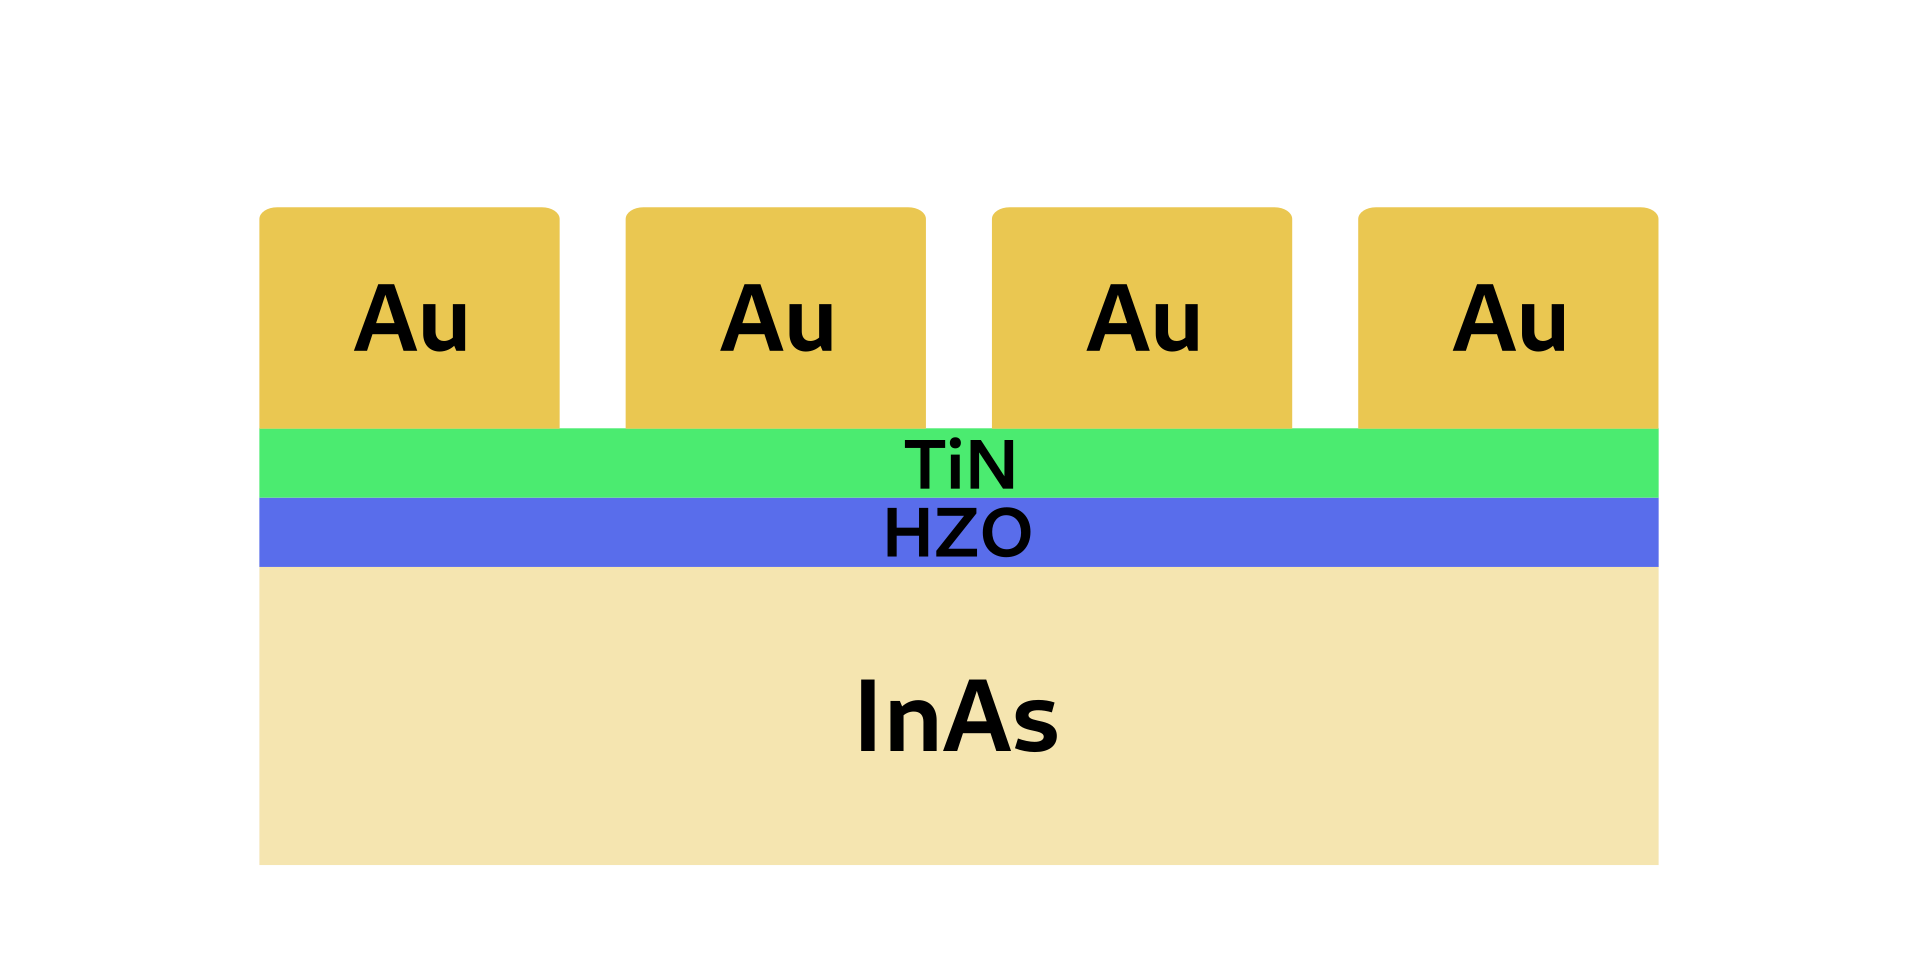
\includegraphics[width=.45\linewidth]{fig/fabproc/fab_4.png}
    \caption{Schematic figure of the sample after device definition and \ce{Au}
    deposition.}\label{fig:fab_4}
\end{figure}

\subsection{Etching of Top Contact}
To further define the devices the \ce{TiN} top contact was etched away in order
to avoid short circuiting. Using a wet-etch in \ce{NH4OH}:\ce{H2O2}:\ce{H2O} at
the ratio of 1:2:5 at \SI{60}{\celsius} the \ce{TiN} was selectively etched
away over a duration of \SI{30}{\second}. Maintaining the samples still in the
wet-etch hindered over-etching and ensured that there was no residue \ce{TiN}
short circuiting the capacitors. Figure \ref{fig:fab_5} shows a schematic of
the finished samples. See figure \ref{fig:fab_babycomp} for a picture of one of
the samples.

\begin{figure}[htbp]
    \centering
    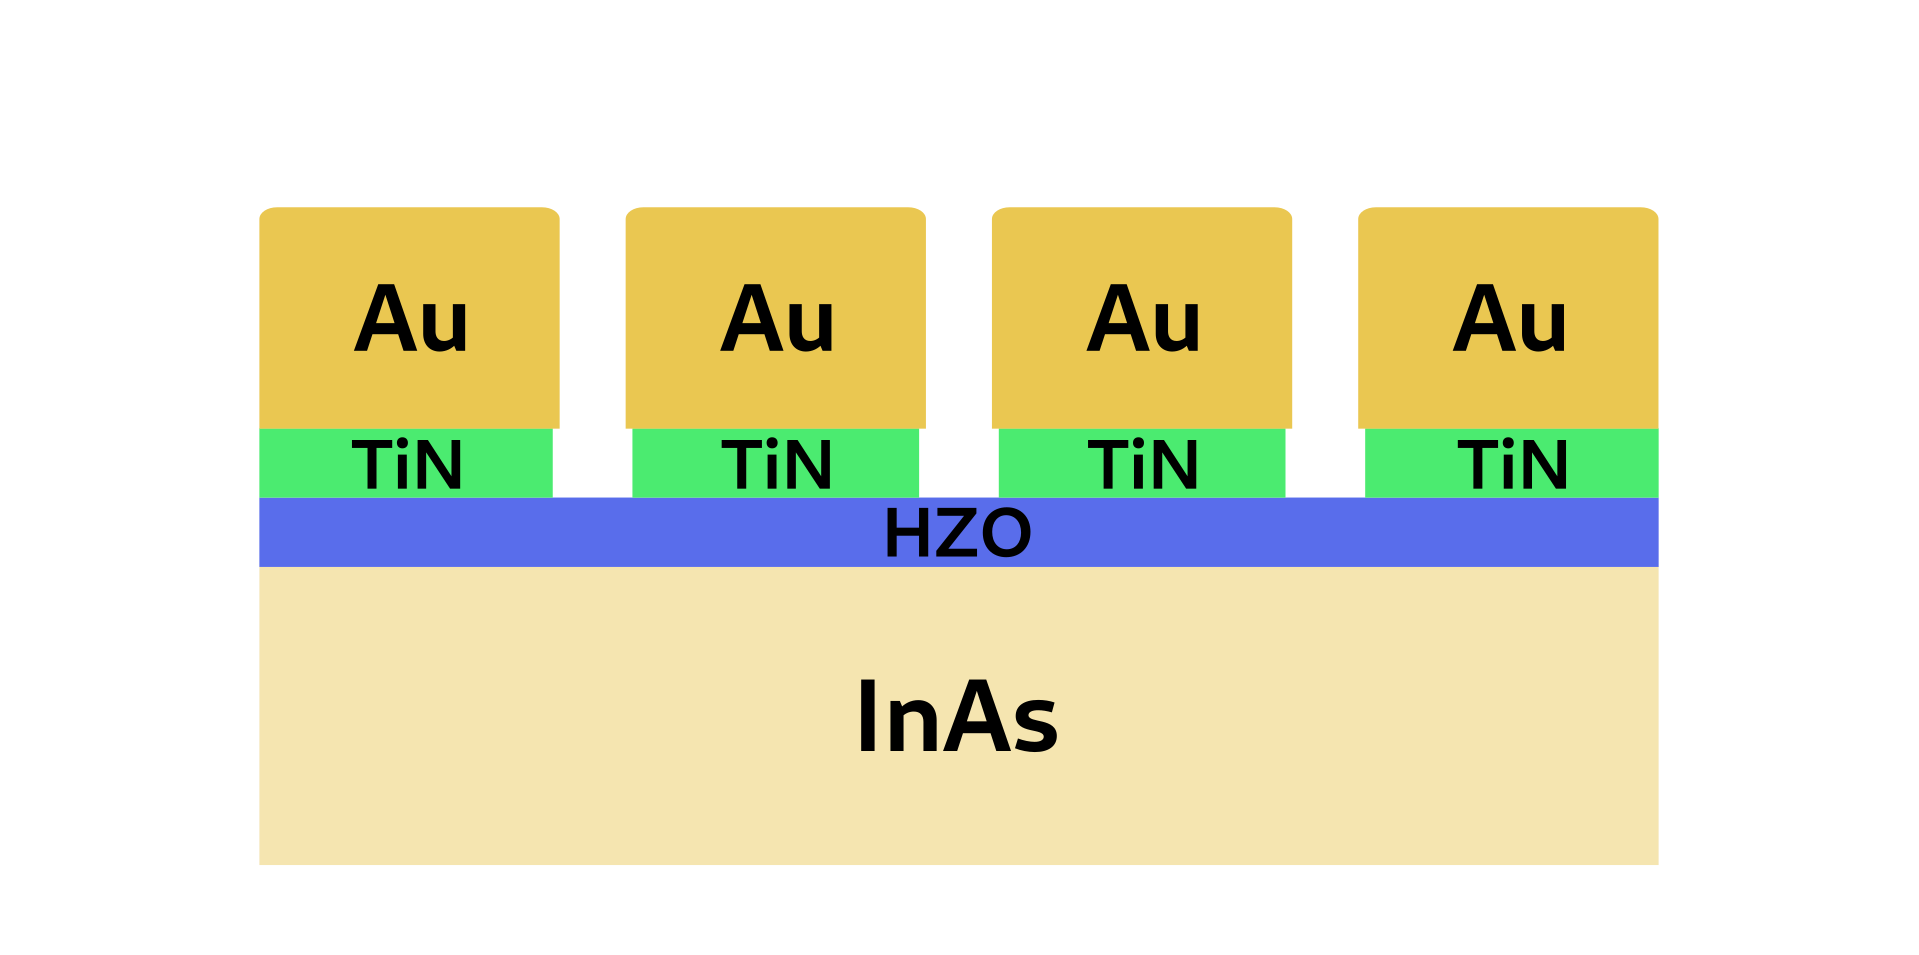
\includegraphics[width=.45\linewidth]{fig/fabproc/fab_5.png}
    \caption{Schematic figure of the sample after top contact etching. This is
    the finished sample.}\label{fig:fab_5}
\end{figure}

To summarize the chapter a step by step schematic of the entire fabrication
process can be seen in figure \ref{fig:fab_done}.

\begin{figure}[htbp]
    \centering
    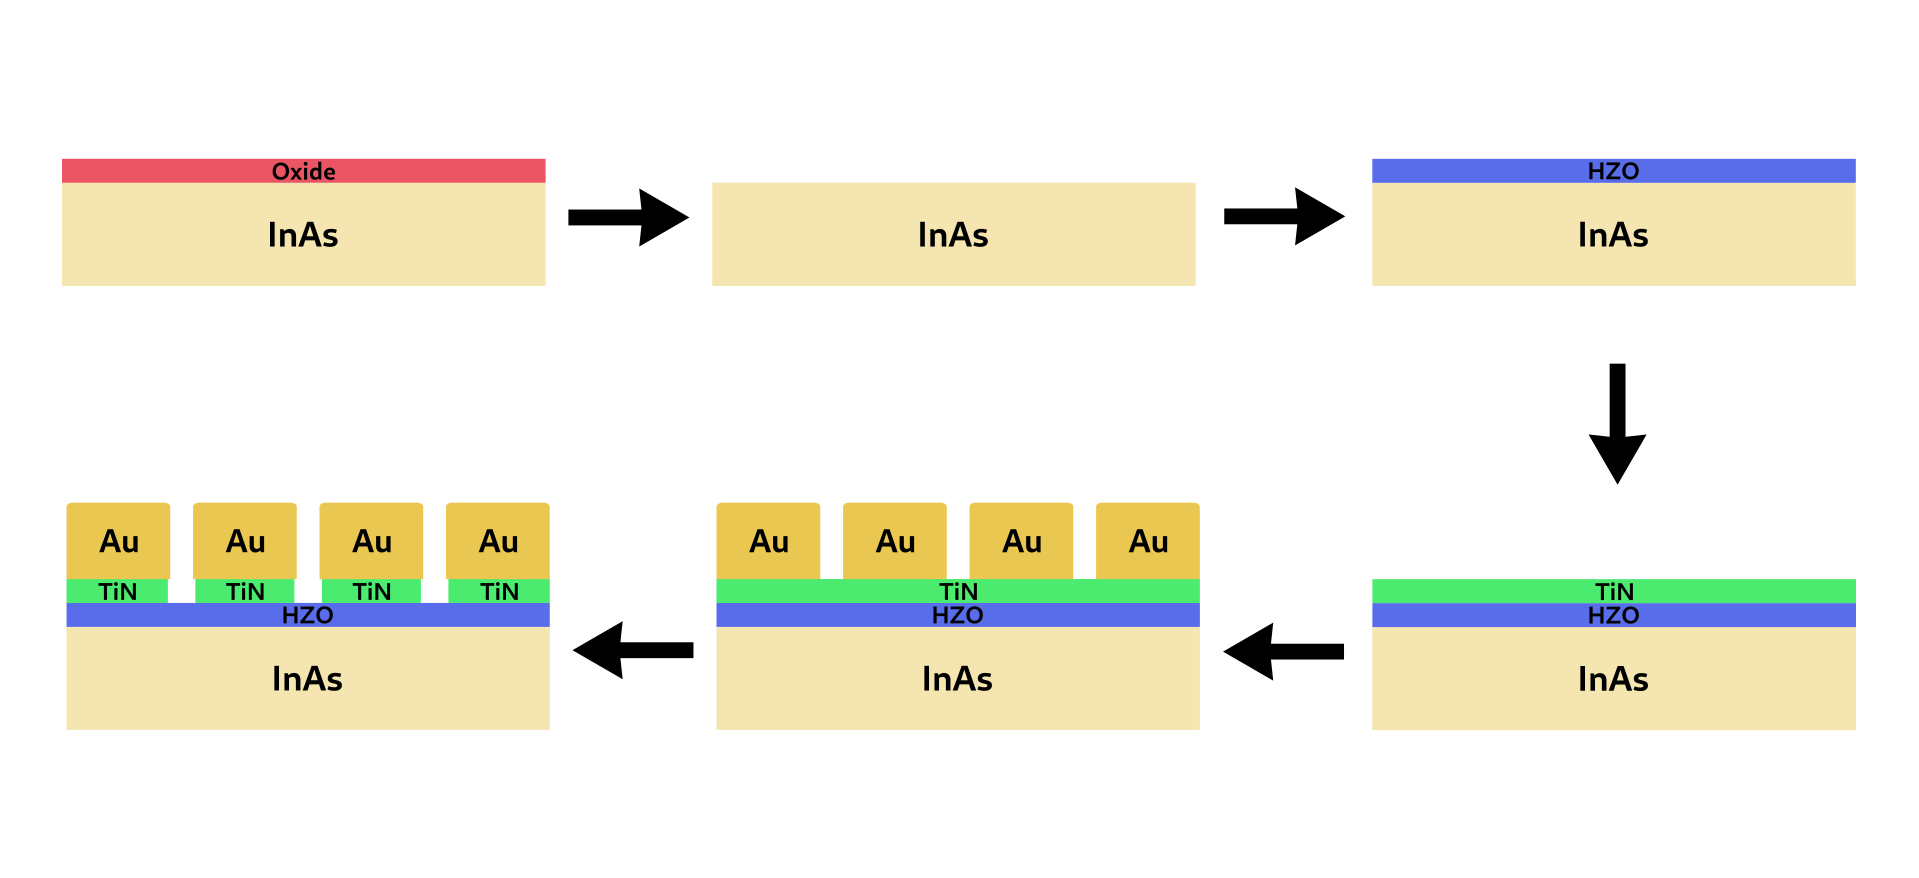
\includegraphics[width=.80\linewidth]{fig/fabproc/fab_done.png}
    \caption{Schematic figure of the entire fabrication process.}\label{fig:fab_done}
\end{figure}

%%%%%%%%%%%%%%%%%%%%%%%%%%
\chapter{Electrical Characterization}\label{ch:char}

Mål: Redogör för metoderna på E-huset.

\section{PUND and Endurance}\label{sec:PandE}

\section{Capacitance-Voltage}\label{sec:CV}

Frågor att besvara: 
\begin{itemize}
    \item Hur funkar metoderna? 
    \item Vilka defekter ser vi med respektive metod? 
\end{itemize}

%%%%%%%%%%%%%%%%%%%%%%%%%%%
\chapter{Results and Analysis}\label{ch:res}

\section{Flashlamp Intensity and Film Temperature}
Crystallization of the hafnia films using the flash lamp annealing (FLA)
technique does not immediately reveal the temperature achieved in the films. Due
to the short time frames and the geometry of the FLA setup, one must simulate
the achieved temperature in the film from the structure of the samples and the
flash parameters. Flash duration and preheating temperature were set to
\SI{5}{\milli\second} and \SI{250}{\celsius} respectively in order to be below
the critical crystallization temperature before the FLA
flash \cite{migita2019phase}. Other simulation parameters are tabulated in
table \ref{tab:app_simparam} and produce figure \ref{fig:res_Comsol} showing the
resulting back and front peak temperature for different pulse energies. The figure also
includes pyrometer measurements of the back temperature during annealing
(green). The discrepancies on the order of \SI{20}{\kelvin} between simulated
back peak temperature (black) and the measured values are attributed to a 
lower reflectivity of the \ce{TiN} capping layer compared to the ideal values of
the simulation. Therefore, the model is deemed to be in reasonable agreement
with the experimental data and gives an estimate of the achieved surface peak temperature.

\begin{figure}[htbp]
    \centering
    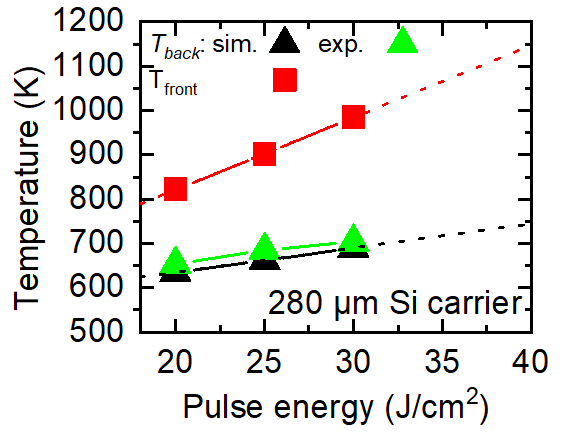
\includegraphics[width=.41\linewidth]{fig/COMSOLFlashInt.png}
    \caption{Simulated back and front peak temperatures of our samples using the
    simulation parameters tabulated in \ref{tab:app_simparam}. Pyrometer
    measurements of the back temperature measured during annealing (green) confirm
    the accuracy of these simulations.}\label{fig:res_Comsol}
\end{figure}

Figure~\ref{fig:res_Comsol} reveal a linear relationship between the pulse
energy ($E_{pulse}$) and the peak HZO film temperature ($T_{peak}$) for our
sample and FLA parameters (eq~\ref{eq:app_filmtemp}). This gives a more
convenient reference going forward using the achieved film temperature rather
than the pulse energy when describing different samples. The usually reported
crystallization temperature required to form the ferroelectric orthorhombic
phase of HZO is in the range of 400-\SI{600}{\celsius}
\cite{muller2012ferroelectricity, athle2022improved}.
The simulated peak surface temperatures in the
20-\SI{30}{\joule\per\square\centi\meter} pulse energy range are significantly
above this critical temperature and should therefore yield a sufficiently high
peak temperature to achieve ferroelectric properties in the HZO.

\section{Sample Specifications and Characterization}
As a reference point, samples were processed using rapid thermal processing
(RTP) as the annealing method in parallel to the FLA samples. These samples
proves as a point of comparison for the characterization of the FLA samples
throughout the work. The RTP samples were annealed at a temperature of
\SI{600}{\celsius} for 30 seconds. The electrical characterization of these
samples, as described in Chapter \ref{ch:char}, were measured and
tabulated in table \ref{tab:res_RTPref}. The remnant polarization and coercive
field are measured after a wakeup of $10^4$ cycles at a pulsing voltage of
\SI{3}{\volt}.

\begin{table}[htbp]
    \caption{Electrical characteristics for the RTP reference samples.}\label{tab:res_RTPref}
    \begin{tabular}{rlrl}
        \toprule
        \multicolumn{4}{c}{PUND, Endurance and Defect Density}\\\midrule
        Remnant Polarization & $P_r$ & $29.03 \pm 0.21$ &
        \si{\micro\coulomb\per\centi\meter\squared}\\
        Coercive Field & $E_c$ & $1.23 \pm 0.18$ &
        \si{\mega\volt\per\centi\meter}\\
        Endurance & & $23 \pm 11$ & $10^3$ cycles\\
        Defect Density & $D_d$ & $9.7 \pm 0.6$ &
        $10^{12}$ \si{\per\centi\meter\squared}
        \\\bottomrule
    \end{tabular}
\end{table}

%TODO: Maybe include here a small paragraph ensuring that all samples (including
%RTP) is fabricated on similar substrates etc? Refering to a table in the
%appendix! Maybe we could ensure the reader in the fabrication section and then
%refirm with a small sentence here.

The processing of the FLA samples are outlined in Section \ref{sec:FabProc}. For
the first FLA series, hereby denoted sample series 1, the flash intensity was
varied between 15-\SI{32.5}{\joule\per\centi\meter\squared} to reach different peak
temperatures in the film. The film deposition and annealing conditions for these
samples are summarized in table \ref{tab:app_IntC}.

Resulting electrical characterization from sample series 1 are shown in
figure \ref{fig:res_IntC}. As seen in figure \ref{fig:res_IntCPr} and
\ref{fig:res_IntCEc} the PUND characteristics show ferroelectric behaviour with
a strong dependence on peak film temperature. The onset of ferroelectricity for
these flashlamp annealed samples seem to be at a peak temperature between
550-\SI{630}{\celsius}. Therefore samples annealed with an intensity less than
\SI{25}{\joule/\centi\meter\squared} are omitted from some of the figures.
The remnant polarization and the coercive fields of these samples follow a similar
pattern reaching a peak of $20.12 \pm 0.59$ \si{\micro\coulomb\per\centi\meter\squared} and a
minimum of $1.46 \pm 0.14$ \si{\mega\volt\per\centi\meter} respectively at a peak
annealing temperature of \SI{711}{\celsius}. Higher temperature annealing
shows a degradation of these ferroelectric properties. %TODO: Why?

Figures \ref{fig:res_IntCPr} and \ref{fig:res_IntCEc} shows that the
described experimental process in Chapter \ref{ch:fab} is indeed a valid process for
fabricating ferroelectric capacitors of this caliber with comparable remnant
polarization and coercive fields to that of samples annealed through RTP.

\begin{figure}[htbp]
    \centering
    \begin{subfigure}{.4\linewidth}
        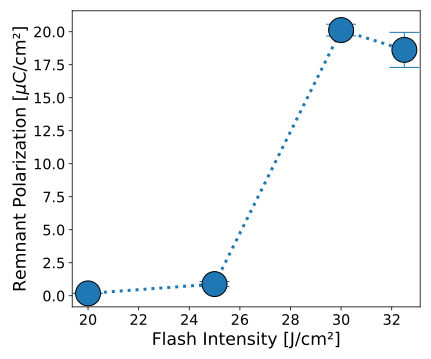
\includegraphics[width=\linewidth]{fig/FlashIntC_PrTrends.png}
        \caption{}\label{fig:res_IntCPr}
    \end{subfigure}
    \begin{subfigure}{.4\linewidth}
        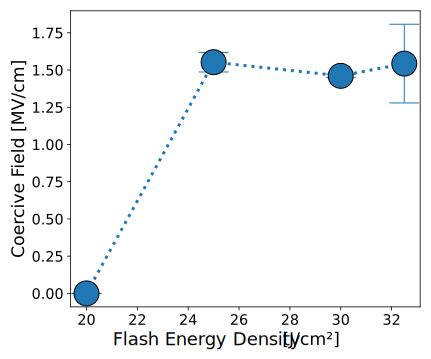
\includegraphics[width=\linewidth]{fig/FlashIntC_EcTrends.png}
        \caption{}\label{fig:res_IntCEc}
    \end{subfigure}
    \begin{subfigure}{.4\linewidth}
        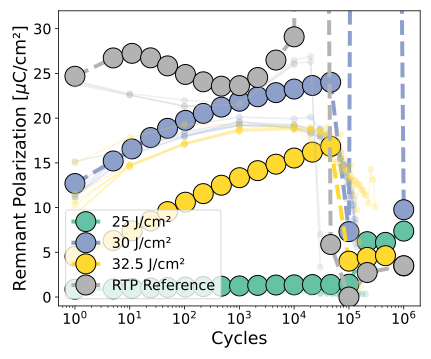
\includegraphics[width=\linewidth]{fig/FlashIntC_EnduTrends.png}
        \caption{}\label{fig:res_IntCEndu}
    \end{subfigure}
    \begin{subfigure}{.4\linewidth}
        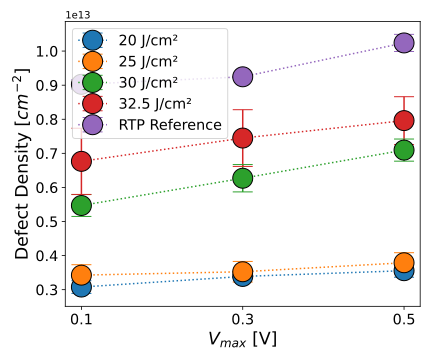
\includegraphics[width=\linewidth]{fig/FlashIntC_DDTrends.png}
        \caption{}\label{fig:res_IntCDD}
    \end{subfigure}
    \caption{Plotted data from sample series 1. Figures a and
        b show the ferroelectric response of the samples at varying peak
        annealing temperature indicating comparable ferroelectric response to
        the RTP annealed samples presented in table \ref{tab:res_RTPref}.
        Figure c and d show improved endurance and reduced defect density
        respectively for all samples annealed through FLA compared to the RTP
        sample.}\label{fig:res_IntC}
\end{figure}

Furthermore, figure \ref{fig:res_IntCEndu} show an increased endurance for
sample series 1 compared to the RTP reference. The comparable sample 4 flashed
with \SI{30}{\joule\per\centi\meter\squared} had a endurance roughly 6 times
greater at values in the range $(127 \pm 13)$ $\cdot 10^3$ cycles. The barely
ferroelectric sample 3 flashed at \SI{25}{\joule\per\centi\meter\squared}
did not breakdown before the measurements ended at $200$ $\cdot 10^3$ cycles and
the endurance of these capacitors should be investigated further to reach a
conclusion for their viability for use in certain gate stacks \cite{dawber2005physics}.
Similarly to $P_r$ and $E_c$, annealing at a higher peak temperature results in degraded
endurance to a value of $(82 \pm 46)$ $\cdot 10^3$ cycles. These values however
are still an improvement compared to the RTP sample.

The improved endurance could be a result of the reduced defect density of the
flash lamp annealed films as shown in figure \ref{fig:res_IntCDD} using the
method described in section \ref{sec:CV}. The measurements reveal a defect
reduction of up to a factor of 3 for sample 3 and close to a factor of 2 for
sample showing comparable $P_r$ and $E_c$ to the RTP sample. This is likely due
to the reduced thermal budget for the FLA samples which generates less initial
defects during the annealing step. However, after sufficiently many cycles the
generated defects (vacancies) start to collect at the \ce{HZO} grain boundaries
increasing the leakage through the oxide and causes the breakdown. However,
the data studied here is not enough to rigorously conclude these theories
\cite{pesic2016physical, athle2022improved}. See table \ref{tab:res_series1} for
a summary of the attained values.

\begin{table}[htbp]
    \caption{Electrical characteristics for sample 4 in sample series
    1. See table \ref{tab:app_IntC} for processing conditions.}\label{tab:res_series1}
    \begin{tabular}{rlrl}
        \toprule
        \multicolumn{4}{c}{PUND, Endurance and Defect Density}\\\midrule
        Remnant Polarization & $P_r$ & $20.12 \pm 0.59$ &
        \si{\micro\coulomb\per\centi\meter\squared}\\
        Coercive Field & $E_c$ & $1.46 \pm 0.14$ & \si{\mega\volt\per\centi\meter}\\
        Endurance & & $127 \pm 13$ & $10^3$ cycles\\
        Defect Density & $D_d$ & $6.1 \pm 0.7$ & $10^{12}$
        \si{\per\centi\meter\squared}
        \\\bottomrule
    \end{tabular}
\end{table}

Although sample series 1 resulted in improved endurance and lower defect density
along with comparable PUND data to the RTP samples, the peak annealing
temperature is still to high in order to significantly reduce the amount of
defects in the film. A closer look at figure \ref{fig:res_IntCDD} and the barely
ferroelectric sample 3 annealed at a flash intensity of
\SI{25}{\joule\per\centi\meter\squared} reveal a further reduction of the defect
density at the cost of ferroelectric response (figure \ref{fig:res_IntCPr}).
Maintaining that low peak annealing temperature over multiple flashes could
result in improved PUND data while not inducing additional defects.

For sample series 2 and 3, tabulated in table \ref{tab:app_NumA} and
\ref{tab:app_NumC} respectively, the number of flashes were varied up to a
maximum of 8 flashes for two different peak annealing temperatures at the onset
of crystallization. The flashes were manually timed at an interval of
approximately \SI{200}{\second}.

Resulting electrical characteristics of sample series 2 and 3 are shown in
figures \ref{fig:res_NumACPUND} and \ref{fig:res_NumACEnduDD}. Figure
\ref{fig:res_NumACPr} reveal an increased ferroelectric response with
additional flashes up to a maximum of $22.98 \pm 1.02$
\si{\micro\coulomb\per\centi\meter\squared} for sample series 2. Sample series 3
on the other hand is not annealed to a significantly high peak temperature to
achieve ferroelectricity until 8 flashes; but even then not to a significant
degree. Sample series 2 show a similar degradation of the ferroelectric response
when flashing up to 8 times as with the increased flash intensity in figure
\ref{fig:res_IntCPr}. % TODO: Same as for IntC, why do we think this is?
The achieved coercive field as shown in figure \ref{fig:res_NumACEc} is
comparable with both sample series 1 and the RTP sample.

\begin{figure}[htbp]
    \centering
    \begin{subfigure}{.4\linewidth}
        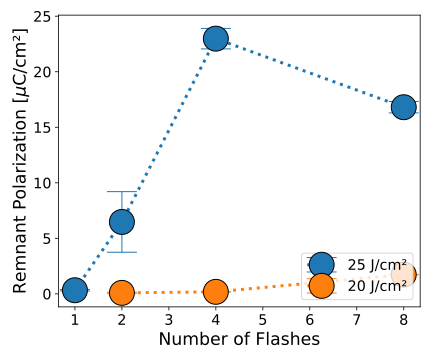
\includegraphics[width=\linewidth]{fig/FlashNumA+C_PrTrends.png}
        \caption{}\label{fig:res_NumACPr}
    \end{subfigure}
    \begin{subfigure}{.4\linewidth}
        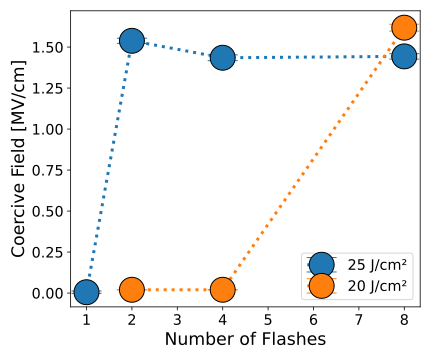
\includegraphics[width=\linewidth]{fig/FlashNumA+C_EcTrends.png}
        \caption{}\label{fig:res_NumACEc}    
    \end{subfigure}
    \caption{Plotted PUND data from sample series 2 and 3. Figure a and b show the
    evolution of the remnant polarization and the coercive field respectively
    over varying number of flashes for two different peak annealing temperatures.
    Increasing the number of flashes with reduced peak annealing temperature
    results in comparable ferroelectric response to the RTP sample as tabulated
    in table \ref{tab:res_RTPref}.}\label{fig:res_NumACPUND}
\end{figure}

Similarly to sample series 1, figure \ref{fig:res_NumACEnduDD} show increased
endurance as well as a lower defect density compared to the RTP sample. Sample 4
of sample series 2 which has the most similar ferroelectric response to the RTP
sample had an endurance in the range $(53 \pm 11)$ $\cdot 10^3$ cycles; an
improvement of a factor of 2. Other samples in the same series showed longer
endurances but at the cost of remnant polarization. More interestingly, the
defect density of sample series 2 shown in figure \ref{fig:res_NumADD} does
increase with multiple flashes reaching a saturated value at 4 flashes an
beyond. This gives indication for the peak annealing temperature of
\SI{630}{\celsius} still being to high in order to avoid the diffusion of
defects in the samples. After 4 flashes the defect density reaches a saturated
value where additional flashes only affects the already generated defects and
assists in the pinning of the domains lowering $P_r$ as shown in figure
\ref{fig:res_IntCPr}.

Sample series 3 does not give any ferroelectric response until the 8th flash as
shown in figure \ref{fig:res_NumACPr}. This is likely due to the low total
thermal impact of the \SI{5}{\milli\second} pulses at this peak annealing
temperature. However, as indicated by figure \ref{fig:res_NumCDD}, the defect
density of these samples also increase with additional flashes, reaching
approximately the same value as for sample series 2 but showing a significantly
lower ferroelectric response. This implies the total energy deposited in the
samples during flashing is enough to induce additional defects but barely enough
to crystallize the HZO to the orthorhombic phase. See table
\ref{tab:res_series2} for a summary of the attained values for sample series 2.
% TODO: Sentance here for why this might be? Could be the cooling and flash rate
% not being quick enough such that the sample spend more time simply collecting
% defects while no crystallization can occur.

\begin{figure}[htbp]
    \centering
    \begin{subfigure}{.4\linewidth}
        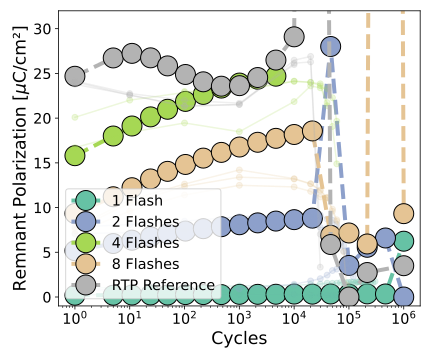
\includegraphics[width=\linewidth]{fig/FlashNumA_EnduTrends.png}
        \caption{}\label{fig:res_NumAEndu}
    \end{subfigure}
    \begin{subfigure}{.4\linewidth}
        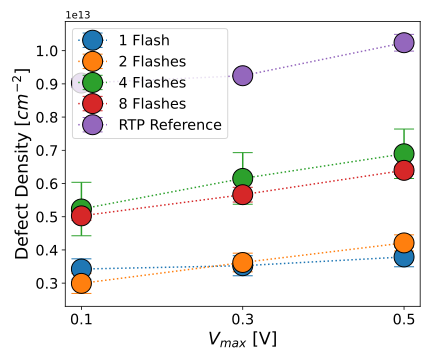
\includegraphics[width=\linewidth]{fig/FlashNumA_DDTrends.png}
        \caption{}\label{fig:res_NumADD}
    \end{subfigure}
    \begin{subfigure}{.4\linewidth}
        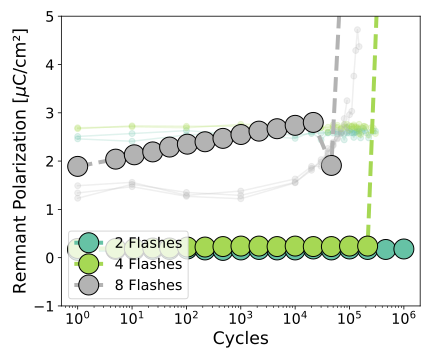
\includegraphics[width=\linewidth]{fig/FlashNumC_EnduTrends.png}
        \caption{}\label{fig:res_NumCEndu}
    \end{subfigure}
    \begin{subfigure}{.4\linewidth}
        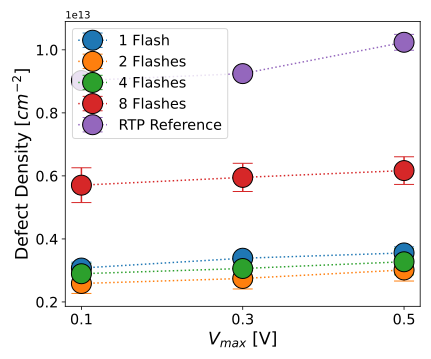
\includegraphics[width=\linewidth]{fig/FlashNumC_DDTrends.png}
        \caption{}\label{fig:res_NumCDD}    
    \end{subfigure}
    \caption{Plotted endurance and defect density from sample series
    2 and 3. Figures a and b show the data from samples series 2 while
    figures c and d show the data from sample series
    3. Increasing the number of flashes with reduced peak annealing temperature
    affects the defect density up to a point where additional flashes only assists
    in pinning the ferroelectric domains. The measured endurance of these samples
    are greater compared to the RTP samples.}\label{fig:res_NumACEnduDD}
\end{figure}

\begin{table}[htbp]
    \caption{Electrical characteristics for sample 3 in sample series
    2. See table \ref{tab:app_NumA} for processing
    conditions.}\label{tab:res_series2}
    \begin{tabular}{rlrl}
        \toprule
        \multicolumn{4}{c}{PUND, Endurance and Defect Density}\\\midrule
        Remnant Polarization & $P_r$ & $22.98 \pm 1.02$ &
        \si{\micro\coulomb\per\centi\meter\squared}\\
        Coercive Field & $E_c$ & $1.44 \pm 0.36$ & \si{\mega\volt\per\centi\meter}\\
        Endurance & & $53 \pm 11$ & $10^3$ cycles\\
        Defect Density & $D_d$ & $5.9 \pm 1.1$ & $10^{12}$
        \si{\per\centi\meter\squared}
        \\\bottomrule
    \end{tabular}
\end{table}

Sample series 1 through 3 show only slight performance improvements to the RTP
samples due to the flash intensity being to high to facilitate additional
crystallization before inducing other effects or the time required for multiple
flashes attributing to an increased defect density without further
crystallization. Both these effects contribute to increased domain pinning and
eventually the breakdown of the individual capacitors. In order to minimize the
energy needed during annealing, one could pre-crystallize the HZO in the ALD
chamber through an increased deposition temperature during growth
\cite{citation needed}.

For sample series 4 and 5, tabulated in table \ref{tab:app_IntE} and
\ref{tab:app_NumD} respectively, the growth temperature during annealing was
increased from \SI{200}{\celsius} to \SI{270}{\celsius}. The HZO growth per
cycle at this elevated temperature is reduced by roughly \SI{20}{\percent} in
our equipment. To compensate for the lower growth per cycle the amount of cycles
was increased to 60:60 to maintain the same HZO thickness as previous samples.

The plotted data from sample series 4 is shown in figure \ref{fig:res_IntE}. The
increased growth temperature does indeed reduce the peak annealing temperature
required to reach the onset of ferroelectricity in the samples as shown in
figure \ref{fig:res_IntEPr}. With the increased growth temperature the window in
which a significant ferroelectric response is achieved is widened and a reduced
coercive field is noted in figure \ref{fig:res_IntEEc}. However, with our
selected peak annealing temperatures it is not clear whether we have surpassed
or yet to have reached the saturation point as noted at a growth temperature of
\SI{200}{\celsius}. It would be interesting to increase the peak annealing
temperature further to see the effects of a higher temperature anneal on the
ferroelectric response.

\begin{figure}[htbp]
    \centering
    \begin{subfigure}{.4\linewidth}
        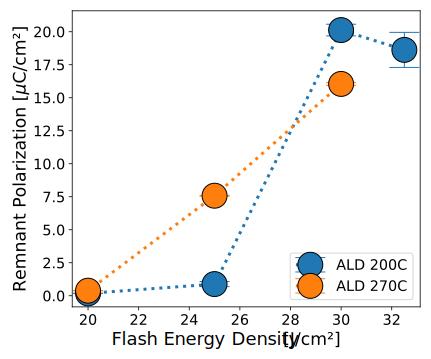
\includegraphics[width=\linewidth]{fig/FlashIntC+E_PrTrends.png}
        \caption{}\label{fig:res_IntEPr}
    \end{subfigure}
    \begin{subfigure}{.4\linewidth}
        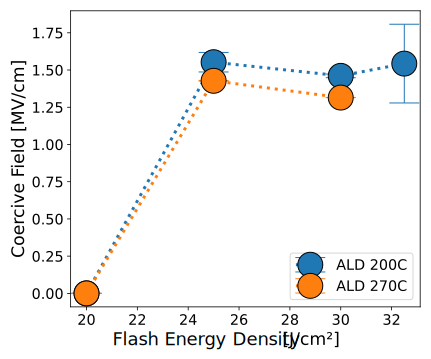
\includegraphics[width=\linewidth]{fig/FlashIntC+E_EcTrends.png}
        \caption{}\label{fig:res_IntEEc}
    \end{subfigure}
    \begin{subfigure}{.4\linewidth}
        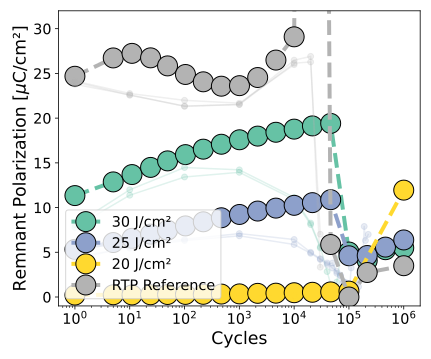
\includegraphics[width=\linewidth]{fig/FlashIntE_EnduTrends.png}
        \caption{}\label{fig:res_IntEEndu}
    \end{subfigure}
    \begin{subfigure}{.4\linewidth}
        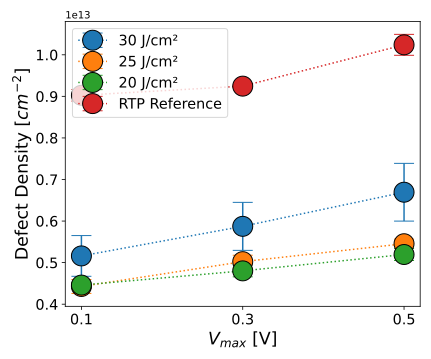
\includegraphics[width=\linewidth]{fig/FlashIntE_DDTrends.png}
        \caption{}\label{fig:res_IntEDD}    
    \end{subfigure}
    \caption{Plotted data from sample series 4. Figures a and b show the
    ferroelectric response of samples grown at different ALD temperatures for
    varying peak annealing temperatures indicating that increasing growth
    temperature assists in lowering the required temperature to reach the onset of
    ferroelectricity. Figure c show improved endurance compared to the RTP
    sample. Figure d shows an overall increase in defect density for samples grown
    at elevated temperature but also a reduced impact of the annealing step on
    defect generation.}\label{fig:res_IntE}
\end{figure}

The endurance of these samples show similar improvement as earlier FLA treated
samples, as seen in figure \ref{fig:res_IntEEndu}. With improvements up to a
factor of five with comparable $P_r$ while samples without significant
ferroelectric response do not reach breakdown $\leq 300\cdot10^3$ cycles. The
increased endurance shows in figure \ref{fig:res_IntEDD} as well through the
reduced defect density of these samples. Interestingly, for these samples an
overall increase in defect density is seen even for samples which do not show
any ferroelectric response. Increasing the peak annealing temperature seem to
have a reduced impact on defect generation and is ultimately comparable with
previous FLA treated samples at a peak annealing temperature of
\SI{711}{\celsius}. This revelation seem to show that the defect generation is
energy dependant and that defects that would be generated by the one
\SI{30}{\joule\per\centi\meter\squared} are being generated during growth
instead. With many defects already generated during growth, the peak annealing
temperature is not high enough to induce additional defects. See table
\ref{tab:res_series4} for a summary of the measured values.

\begin{table}[htbp]
    \caption{Electrical characteristics for sample 3 in sample series
    4. See table \ref{tab:app_IntE} for processing
    conditions.}\label{tab:res_series4}
    \begin{tabular}{rlrl}
        \toprule
        \multicolumn{4}{c}{PUND, Endurance and Defect Density}\\\midrule
        Remnant Polarization & $P_r$ & $16.05 \pm 0.63$ &
        \si{\micro\coulomb\per\centi\meter\squared}\\
        Coercive Field & $E_c$ & $1.32 \pm 0.13$ & \si{\mega\volt\per\centi\meter}\\
        Endurance & & $50 \pm 28$ & $10^3$ cycles\\
        Defect Density & $D_d$ & $5.8 \pm 0.7$ & $10^{12}$
        \si{\per\centi\meter\squared}
        \\\bottomrule
    \end{tabular}
\end{table}

Sample series 4 showed that increasing growth temperature assisted in lowering
the required peak annealing temperature to reach the onset of ferroelectricity
in addition to a reduced impact on defect generation during annealing. However,
to reach significant values of remnant polarization a high peak annealing
temperature is still required. Using the knowledge from sample series 2 and 3 it
might be possible to reduce the impact of annealing on defect generation even
further. 

\begin{figure}[htbp]
    \centering
    \begin{subfigure}{.4\linewidth}
        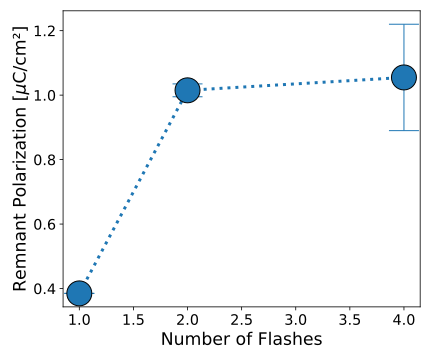
\includegraphics[width=\linewidth]{fig/FlashNumD_PrTrends.png}
        \caption{}\label{fig:res_NumDPr}
    \end{subfigure}
    \begin{subfigure}{.4\linewidth}
        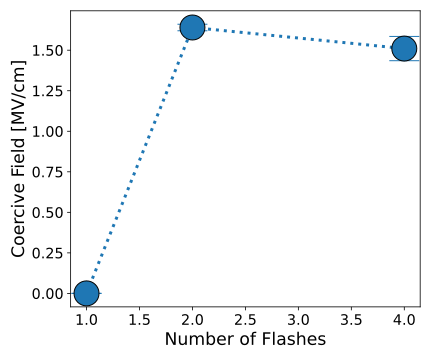
\includegraphics[width=\linewidth]{fig/FlashNumD_EcTrends.png}
        \caption{}\label{fig:res_NumDEc}
    \end{subfigure}
    \begin{subfigure}{.4\linewidth}
        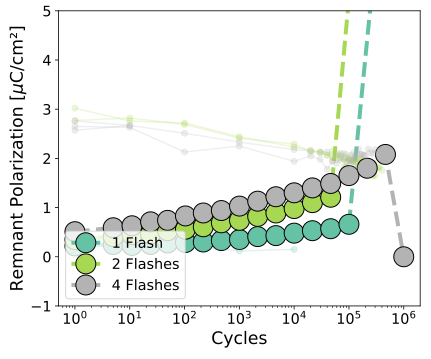
\includegraphics[width=\linewidth]{fig/FlashNumD_EnduTrends.png}
        \caption{}\label{fig:res_NumDEndu}
    \end{subfigure}
    \begin{subfigure}{.4\linewidth}
        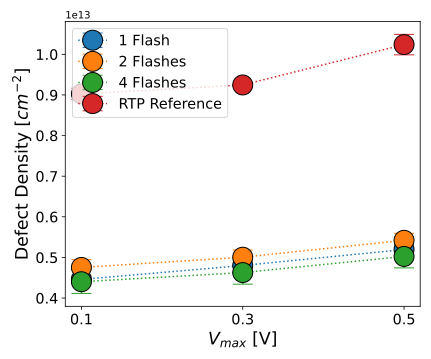
\includegraphics[width=\linewidth]{fig/FlashNumD_DDTrends.png}
        \caption{}\label{fig:res_NumDDD}    
    \end{subfigure}
    \caption{Plotted data from sample series 5. Figures a and b show the
    ferroelectric response of the samples annealed at a peak annealing
    temperature of \SI{548}{\celsius} over varying number of flashes. The figures
    reveal that the temperature is not high enough to reach the onset of
    ferroelectricity despite having been grown at an elevated ALD temperature.
    Figure c shows the supposed endurance that is only affects by the increasing
    leakage current during cycling. Figure d affirms the higher defect density of
    samples grown at the elevated growth temperature and shown no effect on defect
    generation throughout the annealing steps.}\label{fig:res_NumD}
\end{figure}

The plotted data from sample series 5 is shown in figure \ref{fig:res_NumD}. The
peak annealing temperature for these samples are \SI{548}{\celsius} in the
attempt to incrementally reach the onset of ferroelectricity with additional
flashes. Figures \ref{fig:res_NumDPr} and \ref{fig:res_NumDEc} show $P_r$ and
$E_c$ respectively and reveal that the peak annealing temperature is not
sufficient to reach the onset of ferroelectricity for up to 4 flashes. Although
some response is measured for all samples, this is attributed to the noisiness
of non-ferroelectric samples. Since the samples are not ferroelectric, the
endurance in figure \ref{fig:res_NumDEndu} show only an increasing remnant
polarization response due to increased leakage current during cycling. Figure
\ref{fig:res_NumDDD} show the same elevated defect density as in figure
\ref{fig:res_IntEDD} which stay consistent throughout annealing.

%%%%%%%%%%%%%%%%%%%%%%%%%%
\chapter{Conclussion}\label{chap:conc}

This report shows successful integration of ferroelectric HZO into a
\ce{InAs}/\ce{HZO}/\ce{TiN} stack using a flash lamp annealing (FLA) technique. The
resulting capacitors show comparable ferroelectric response with capacitors
annealed through rapid thermal processing (RTP) with an improved endurance up
to a factor 5. The improved endurance is attributed to the reduced defect
density of the films processed using FLA. This in part due to the reduced
thermal budget of the FLA technique which reduces the diffusion of oxygen
vacancies as well as the formation of \ce{As} and \ce{In} oxides from the
substrate.\cite{kang2016structural} The reduced defect density allows for
additional endurance cycling before breakdown of the ferroelectric capacitor.

In our efforts of further reducing the defect density, both multiple flashes at
a lower peak annealing temperature and pre-crystallization during growth was
examined. However, these efforts showed varied success. Additional flashes
showed only marginal improvements up to the amount of flashes tested during
these experiments. Using a flash lamp annealer which can produce multiple
flashes at a higher repetition rate could prove fruitful. Pre-crystallization
of the HZO during growth showed marginal success in lowering the required peak
annealing temperature to reach the onset of ferroelectricity but did in itself
prove detrimental to the defect density of the samples.

In order to better understand the material effects of these efforts this data
could be combined with studies of the oxide bulk and surface to identify
defects and their properties. In a complementary study by R. Athle et al the
data from this study is combined with XPS data to better understand the
defects of the samples.\cite{athle2022improved}

%%%%%%%%%%%%%%%%%%%%%%%%%%%%%%%%%%%%%%%
%% References
\bibliography{Exjobbreport.bib}
\bibliographystyle{ieeetr}


%%%%%%%%%%%%%%%%%%
\appendix
%%%%%%%%%%%%%%%%%%%
\chapter{Extra Material}\label{app:extra}
\begin{table}[htbp]
    \centering
    \caption{Relevant simulation parameters used in COMSOL to achieve
    figure~\ref{fig:res_Comsol}. The \ce{InAs/HZO/TiN} is part of the sample
while \ce{Si} is a carrier wafer part of the FLA experimental setup.}\label{tab:app_simparam}
    \begin{tabular}{crcc}
        \toprule
        Layer & Thickness & Doping & Reflectivity \\\midrule
        \ce{TiN} & \SI{10}{\nano\meter} &~- & 0.41 \\ 
        \ce{HZO} & \SI{10}{\nano\meter} & 1:1 (\ce{Hf/Zr}) &~- \\ 
        \ce{InAs} & \SI{280}{\micro\meter} & \SI{1e16}{\per\centi\meter\tothe{3}} &~- \\ 
        \ce{Si} & \SI{280}{\micro\meter} &~- &~- \\\bottomrule
    \end{tabular}
\end{table}

\begin{equation}\label{eq:app_filmtemp}
    T_{peak} [\si{\kelvin}] = 495.5 + 16.3 \cdot E_{pulse} [\si{\joule\per\square\centi\meter}]
\end{equation}

\chapter{Processing Parameters}\label{app:procparam}
\begin{table}[htbp]
    \caption{Selected processing conditions for sample series 1.}\label{tab:app_IntC}
    \begin{tabular}{rlccccc}
        \toprule
        \multicolumn{2}{l}{Sample Number} & 1 & 2 & 3 & 4 & 5 \\\midrule
        \multicolumn{1}{c}{HZO} & & & & & & \\
        Growth Temperature & [\si{\celsius}] & 200 & 200 & 200 & 200 & 200 \\
        Deposition Cycles & [\ce{Hf}:\ce{Zr}] & 50:50 & 50:50 & 50:50 & 50:50 & 50:50 \\\midrule
        \multicolumn{1}{c}{FLA} & & & & & & \\
        Preheat Temperature & [\si{\celsius}] & 250 & 250 & 250 & 250 & 250 \\
        Peak Temperature & [\si{\celsius}] & \textbf{467} & 
        \textbf{548} & \textbf{630} & \textbf{711} & \textbf{752} \\
        Number of Flashes & & 1 & 1 & 1 & 1 & 1 \\\bottomrule
    \end{tabular}
\end{table}

\begin{table}[htbp]
    \caption{Selected processing conditions for sample series
    2.}\label{tab:app_NumA}
    \begin{tabular}{rlcccc}
        \toprule
        \multicolumn{2}{l}{Sample Number} & 1 & 2 & 3 & 4 \\\midrule
        \multicolumn{1}{c}{HZO} & & & & & & \\
        Growth Temperature & [\si{\celsius}] & 200 & 200 & 200 & 200 \\
        Deposition Cycles & [\ce{Hf}:\ce{Zr}] & 50:50 & 50:50 & 50:50 & 50:50 \\\midrule
        \multicolumn{1}{c}{FLA} & & & & & \\
        Preheat Temperature & [\si{\celsius}] & 250 & 250 & 250 & 250 \\
        Peak Temperature & [\si{\celsius}] & 630 & 630 & 630 & 630 \\
        Number of Flashes & & \textbf{1} & \textbf{2} & \textbf{4} & \textbf{8} \\\bottomrule
    \end{tabular}
\end{table}

\begin{table}[htbp]
    \caption{Selected processing conditions for sample series
    3.}\label{tab:app_NumC}
    \begin{tabular}{rlccc}
        \toprule
        \multicolumn{2}{l}{Sample Number} & 1 & 2 & 3 \\\midrule
        \multicolumn{1}{c}{HZO} & & & & \\
        Growth Temperature & [\si{\celsius}] & 200 & 200 & 200 \\
        Deposition Cycles & [\ce{Hf}:\ce{Zr}] & 50:50 & 50:50 & 50:50 \\\midrule
        \multicolumn{1}{c}{FLA} & & & & \\
        Preheat Temperature & [\si{\celsius}] & 250 & 250 & 250 \\
        Peak Temperature & [\si{\celsius}] & 548 & 548 & 548 \\
        Number of Flashes & & \textbf{2} & \textbf{4} & \textbf{8} \\\bottomrule
    \end{tabular}
\end{table}

\begin{table}[htbp]
    \caption{Selected processing conditions for sample series
    4.}\label{tab:app_IntE}
    \begin{tabular}{rlccc}
        \toprule
        \multicolumn{2}{l}{Sample Number} & 1 & 2 & 3 \\\midrule
        \multicolumn{1}{c}{HZO} & & & & \\
        Growth Temperature & [\si{\celsius}] & 270 & 270 & 270 \\
        Deposition Cycles & [\ce{Hf}:\ce{Zr}] & 60:60 & 60:60 & 60:60 \\\midrule
        \multicolumn{1}{c}{FLA} & & & & \\
        Preheat Temperature & [\si{\celsius}] & 250 & 250 & 250 \\
        Peak Temperature & [\si{\celsius}] & \textbf{548} & \textbf{630} &
        \textbf{711} \\
        Number of Flashes & & 1 & 1 & 1 \\\bottomrule
    \end{tabular}
\end{table}

\begin{table}[htbp]
    \caption{Selected processing conditions for sample series
    5.}\label{tab:app_NumD}
    \begin{tabular}{rlccc}
        \toprule
        \multicolumn{2}{l}{Sample Number} & 1 & 2 & 3 \\\midrule
        \multicolumn{1}{c}{HZO} & & & & \\
        Growth Temperature & [\si{\celsius}] & 270 & 270 & 270 \\
        Deposition Cycles & [\ce{Hf}:\ce{Zr}] & 60:60 & 60:60 & 60:60 \\\midrule
        \multicolumn{1}{c}{FLA} & & & & \\
        Preheat Temperature & [\si{\celsius}] & 250 & 250 & 250 \\
        Peak Temperature & [\si{\celsius}] & 548 & 548 & 548 \\
        Number of Flashes & & \textbf{1} & \textbf{2} & \textbf{4} \\\bottomrule
    \end{tabular}
\end{table}

\end{document}
